\section{Podstawowe informacje dotyczące przetwarzania obrazów}
\subsection{Podstawowe definicje}
\subsubsection{Piksel}
Piksel jest najmniejszym elementem obrazu cyfrowego. Piksel może określać
\begin{itemize}
\item odcień szarości
\item kolor, wtedy \(f(x, y) = [a(x, y), b(x, y),...]\)\\
  gdzie $a, b,...$ to natężenie poszczególnych barw
\item wskaźnik na element tablicy barw
\end{itemize}
\subsubsection{Obraz cyfrowy}
Obraz cyfrowy jest macierzą pikseli, postaci
\begin{gather*}
  f = f(x, y), x = 0,1,2,...,N-1; y = 0,1,2,...,M-1
\end{gather*}
gdzie
\begin{itemize}
\item \(f(x, y)\) - pojedynelement macierzy, piksel
\item \(M, N\) - szerokość oraz wysokość obrazu
\end{itemize}
\subsubsection{Obraz binarny}
Obraz binarny jest to obraz cyfrowy którego składowe piksele przyjmują wartości
\begin{gather*}
  f(x, y) = z, z \in {0, 1}
\end{gather*}.
\subsection{Podstawowe algorytmy przetwarzania obrazów}
\subsubsection{Operacje morfologiczne}
Operacje morfologiczne na obrazach binarnych wykoszystywane są do filtracji morfologicznej oraz analizy kształtów obiektów na obrazie. Algorytmy morfologiczne są podstawą dla wielu bardziej złożonych algorytmów analizy wizji komputerowej.
\paragraph {Dylatacja obrazu} to rozszerzenie obrazu element strukturalny. Operacja definiowana jest wzorem
\begin{gather*}
  A \bigoplus B \equiv \bigcup \limits_{b \in B} A_b
\end{gather*}.
Przykładowy wynik operacji dylatacji przedstawiony jest na rysunku~\ref{fig:dilate}.
\begin{figure}
  \centering
  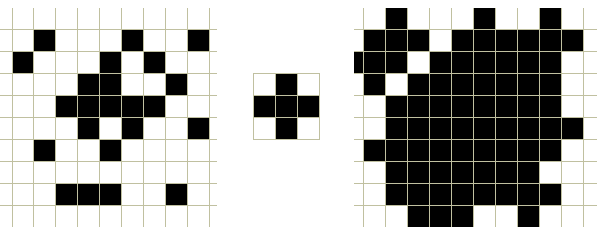
\includegraphics[width=15.5cm]{img/dilate}
  \caption{Obraz binarny poddany procesowi dylatacji z zadanym elementem strukturalnym}
  \label{fig:dilate}
\end{figure}
